\section{Concurrent Insertion and Analytics}
\label{sec:eval:dynamic:concurrent}
\newflag[entire section is new]

Every experiment so far separates writing from reading.
\autoref{sec:eval:dynamic} ingests a graph and then analyses it.
This section runs both at once, and that is where \project{}'s central design decision meets its most challenging workload.
\project{} gives an analytics pass a consistent view of the graph by running it against a checkpoint, so that every kernel in the pass traverses the same graph however much the writers change underneath it.
Producing that checkpoint means writing out the B-trees that hold the graph, and the writers keep modifying those same trees while it is written.
The two contend on every tree they share, and how much they contend follows from how a layout distributes the graph across B-trees.
EdgeKey, the layout we measure here, keeps almost all of the graph in a single edge table.

\subsection{Workload and metrics}
\label{sec:eval:dynamic:concurrent:setup}

We replay the \texttt{graph500-24} update log with $W$ writer threads.
The remaining $R = 50 - W$ threads of a $50$-thread budget run analytics passes over a checkpoint, one pass after another.
An \emph{analytics pass} runs BFS, PageRank, WCC, SSSP, and the one- and two-hop neighbour queries in a fixed order.
Analytics begins once the writers have replayed a tenth of the log, so every pass reads a graph that is already large and still growing.

We report three quantities: how many checkpoints a run produced, how long each one took, and how much throughput the writers sustained while analytics ran.
We summarise the last as \emph{retention}, the mean writer throughput during the analytics window divided by the mean before analytics began.
Both rates come from the same run, so retention separates what analytics costs the writers from the rate those writers reach on their own.
We call a writer \emph{stalled} when its throughput falls below $5$\,K\,ops/s, roughly $2\%$ of the rate reached before analytics at $W=5$, and we report the share of the analytics window spent that way.

\project{} runs the EdgeKey layout with an $800$\,GiB cache and the write-ahead log switched off.
\wt{}'s background checkpoint server runs throughout, at the interval set by \texttt{checkpoint=(wait=$N$)}, and $N$ is $10$\,s unless we say otherwise.
All experiments in this section were run on Machine A (\autoref{tab:eval-hardware}).

Eviction runs at \wt{}'s default thresholds, the right-hand column of \autoref{tab:wt-eviction-knobs}.
\autoref{sec:eval:dynamic:dirty} raised \texttt{eviction\_dirty\_target} and \texttt{eviction\_dirty\_trigger} to $85\%$ and $95\%$ instead, which lets the cache absorb almost every dirty page; eviction wrote nothing at all for the first $31$ minutes of that experiment.
This workload cannot run that way.
Analytics runs for hours, and the writers need eviction reclaiming pages throughout.

\wt{} tracks two quantities here, each with its own thresholds.
\emph{Dirty data} is the bytes in pages whose images a checkpoint or an eviction must write out.
\emph{Update bytes} counts only the in-memory update chains that \project{} appends to on every edge insertion, not the page images that hold them, and its thresholds are derived as half the dirty ones.
On our $800$\,GiB cache that puts \texttt{eviction\_updates\_trigger} at $80$\,GiB, and it is the threshold that binds in this workload.
Once update bytes cross that threshold, \wt{} conscripts application threads into performing eviction themselves.

\subsection{A fresh checkpoint for every analytics pass stalls the writers}
\label{sec:eval:dynamic:concurrent:forced}

The obvious implementation forces a new checkpoint at the start of each analytics pass, in addition to the ones the background server is already taking.
The goal is not to hand the pass the latest view of the graph: reading the live table would do that, but would let a kernel watch the graph change under it as the writers commit.
Analytics needs a consistent and durable view of the graph and can tolerate bounded staleness.
Taking a fresh checkpoint at the beginning of each analytics pass keeps that staleness as small as it can be.
The choice, however, also stalls the writers almost completely.
At $W=25$ each pass waits between $432$ and $625$ seconds for its checkpoint, the writers stall for $88.5\%$ of the analytics window, and they retain only $10.3\%$ of their pre-analytics rate (\autoref{fig:concurrent-forced}, top).

Recall that in this experiment \wt{}'s checkpoint server is active and produces checkpoints on its own schedule.
Pointing the readers at that rolling checkpoint, rather than forcing a new one, removes the wait from the analytics path.
Measured in the same session and on the same data, retention rises to $60.8\%$, and a pass finishes in $39$ to $108$ seconds rather than in the $445$ to $690$ a forced pass takes, almost all of it spent waiting (\autoref{fig:concurrent-forced}, bottom).

That $60.8\%$ retention comes from averaging three passes that run near the writers' pre-analytics rate with two during which writer throughput is exactly zero.
The fourth and the fifth pass are the ones where the writers are stalled; these account for $31.6\%$ of this run's five-pass analytics window, which is only $271$ seconds long.

%%%%%%%%%%%%%%%%%%%%%%%%%%%%%%%%%%%%%%%%%%%%%%%%%%%%%%%%%%%%%%%%%%%%%%%%%%%%%%%%
\begin{figure}[!htb]
  \centering
  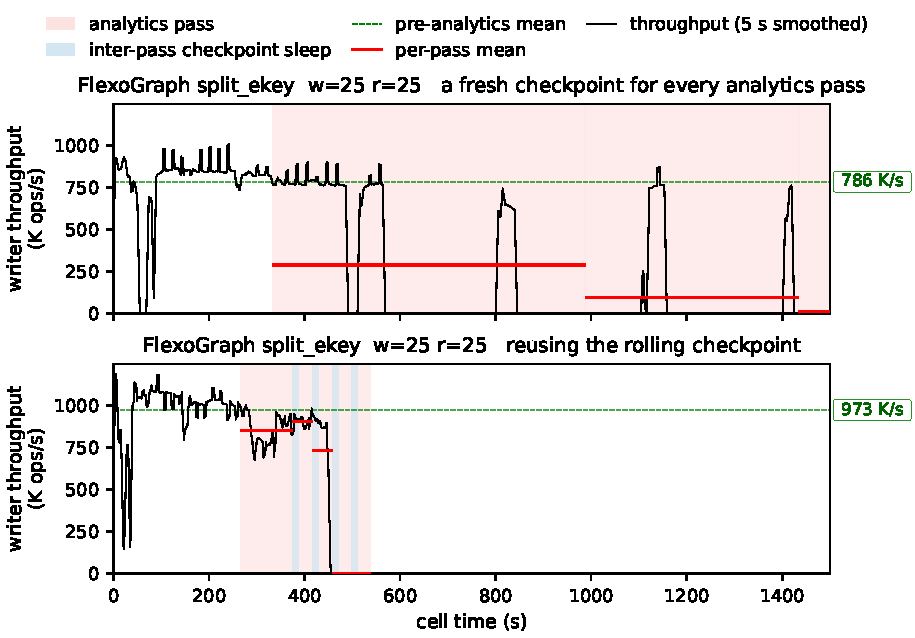
\includegraphics[width=\columnwidth]{fig/dynamic/concurrent_forced_vs_reuse.pdf}
  \caption{Writer throughput at $W=25$ under the two policies, measured in the same session and drawn on one time axis, cut at $1{,}500$ seconds.
  Both runs perform five analytics passes.
  The configuration that reuses the default WiredTiger checkpoint (bottom) completes all five by $546$ seconds, where its run ends and its panel goes blank. In the configuration in which we explicitly force a checkpoint before each analytics task is still in its first pass at that point, and in its third where the figure ends.
  These explicit checkpoints reduce writer throughput to a mean value of $290$\,K\,ops/s in the first pass and $95$\,K\,ops/s in the second pass, and the recoveries between checkpoints are the only work they get done.
  With these explicit checkpoints the analytics window consumes $3{,}367$ seconds, and its last three passes average $10.6$, $5.0$ and $5.3$\,K\,ops/s.
  Reusing WiredTiger's default checkpoints keeps the writers near their own mean for three passes, but the fourth and fifth stop them completely, so its $60.8\%$ retention averages three live passes with two dead ones.
  The two runs also start from different pre-analytics rates, which the policy cannot account for because it takes effect only once analytics begins; each curve is therefore read against its own dashed line and not against the other panel.}
  \label{fig:concurrent-forced}
\end{figure}
%%%%%%%%%%%%%%%%%%%%%%%%%%%%%%%%%%%%%%%%%%%%%%%%%%%%%%%%%%%%%%%%%%%%%%%%%%%%%%%%

Reuse delays the stalls; it does not prevent them.
\wt{}'s checkpoint server still runs on its own schedule over the same edge table the writers are modifying, and \autoref{sec:eval:dynamic:concurrent:mechanism} examines why that eventually stalls the writers.

\subsection{Why the writers stall}
\label{sec:eval:dynamic:concurrent:mechanism}

The obvious response is to give the checkpoint less to contend with.
Every writer thread adds to the dirty data that a checkpoint must write out and that eviction must reclaim, so cutting the count from $25$ writers to $5$ slows the rate at which it builds up.
The rest of this section runs at $W=5$ unless we say otherwise, and returns to $W=25$ where a faster collapse makes a mechanism easier to observe.
It buys time, and only time: the first analytics pass that stalls the writers now arrives twenty-eight minutes into the analytics window rather than three.
\autoref{fig:concurrent-collapse} shows twenty passes at the default $10$\,s checkpoint interval: $W=5$ retains $39.3\%$ of its pre-analytics throughput across a $78.6$-minute window, stalls for $48.2\%$ of it, and loses $305$ seconds to a single stall.
In comparison, $W=25$ retained only $11.8\%$ of its own pre-analytics throughput over the same twenty passes, which took $54.4$ minutes at that writer count.
A fixed pass count is therefore not a fixed duration, and the runs that follow are bounded by elapsed time instead.

%%%%%%%%%%%%%%%%%%%%%%%%%%%%%%%%%%%%%%%%%%%%%%%%%%%%%%%%%%%%%%%%%%%%%%%%%%%%%%%%
\begin{figure}[!htb]
  \centering
  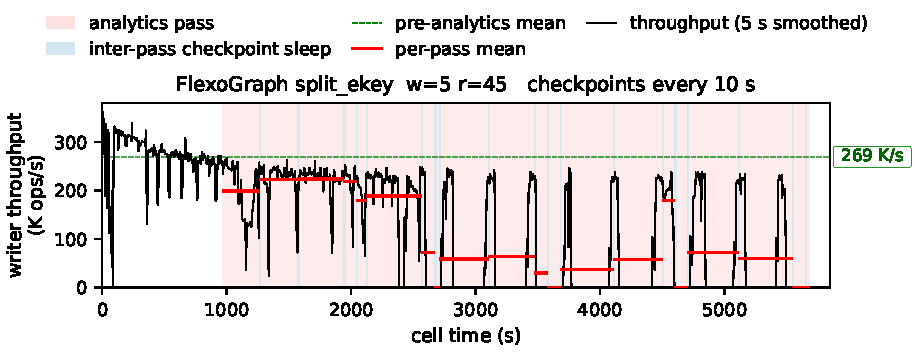
\includegraphics[width=\columnwidth]{fig/dynamic/concurrent_collapse.pdf}
  \caption{Writer throughput at $W=5$ across twenty analytics passes at the default $10$\,s checkpoint interval.
  The first six passes hold between $67$ and $83\%$ of the pre-analytics mean.
  From the seventh onwards no pass exceeds $27\%$ except one at $66\%$, and through five of the last fourteen the writers do no work at all.
  The decay is not a steady slope but a lengthening of the stalls.}
  \label{fig:concurrent-collapse}
\end{figure}
%%%%%%%%%%%%%%%%%%%%%%%%%%%%%%%%%%%%%%%%%%%%%%%%%%%%%%%%%%%%%%%%%%%%%%%%%%%%%%%%

A $9.2$-hour run at $W=25$ shows where this ends.
Writer throughput decays from $409$\,K\,ops/s to $5.9$\,K\,ops/s.
Over the same period a checkpoint runs for $97.2\%$ of the wall-clock, and the writers spend $90\%$ of their thread-time waiting for cache.
No pass makes exactly zero progress, because throughput reads zero only while the writers are conscripted and no pass is conscripted for its whole duration, so the decay is asymptotic rather than terminal.

While \wt{} checkpoints a B-tree, it forbids the eviction of that tree's dirty pages.
The rule protects correctness: evicting a dirty child after its parent has already been written would leave an inconsistent checkpoint.
EdgeKey holds almost all of the graph in one edge table, so this rule bars eviction almost everywhere, almost all of the time.
A checkpoint's duration depends on how much dirty data it must write.
The $9.2$-hour run took $93$ checkpoints that varied in how long \wt{} needed to create them: the first five grew from $8$ to $149$ seconds, and the remaining $88$ then held between $314$ and $412$ seconds for eight hours, because the dirty data each one had to write stayed between $84$ and $89$\,GiB for the whole of that time.

Barred eviction keeps dirty data high, and update bytes climb with it.
Once they reach the $80$\,GiB \texttt{eviction\_updates\_trigger}, \wt{} conscripts the application threads into performing eviction themselves.
Those threads find nothing they may evict, and they wait without a timeout.
Writer throughput then reads exactly zero, and the longest single insert latency matches the length of the stall.
\autoref{fig:concurrent-dirty} traces update bytes at two checkpoint intervals: \wt{}'s $10$\,s default and the $120$\,s setting of \autoref{sec:eval:dynamic:concurrent:spaced}.
At $10$\,s update bytes reach the $80$\,GiB threshold and stay there; at $120$\,s they never reach it.

%%%%%%%%%%%%%%%%%%%%%%%%%%%%%%%%%%%%%%%%%%%%%%%%%%%%%%%%%%%%%%%%%%%%%%%%%%%%%%%%
\begin{figure}[!htb]
  \centering
  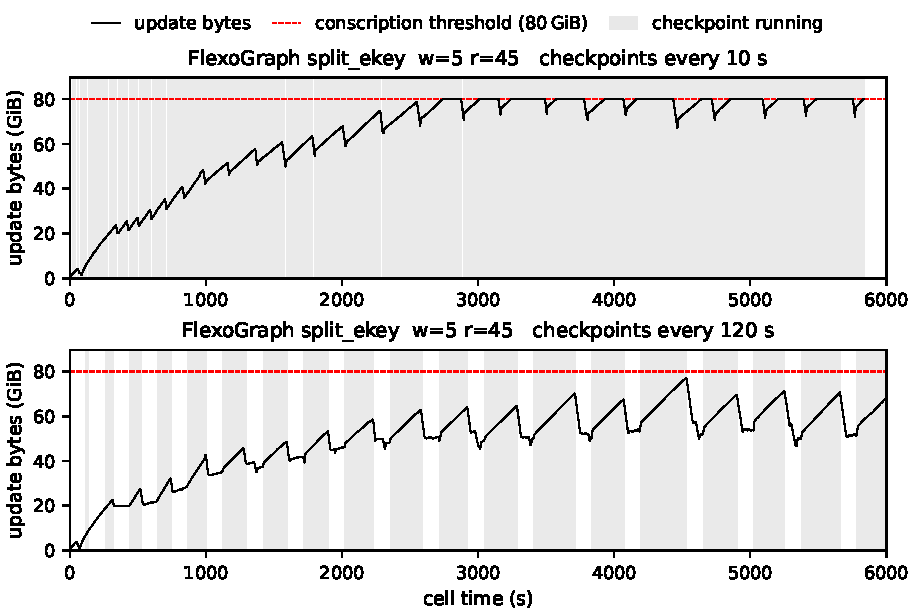
\includegraphics[width=\columnwidth]{fig/dynamic/concurrent_dirty.pdf}
  \caption{Update bytes at $W=5$, against \texttt{eviction\_updates\_trigger}, the level at which \wt{} conscripts writer threads into eviction.
  The grey bands mark when a checkpoint is running.
  The curve climbs inside each band, where the checkpoint bars eviction, and drains between bands; that alternation is what gives the trace its teeth.
  At the default $10$\,s checkpoint interval the gaps drain almost nothing: update bytes climb for $45$ minutes, reach the $80$\,GiB threshold and stay on it, holding the writers at exactly the point where conscription begins.
  At a $120$\,s checkpoint interval each fall undoes the rise before it, and they peak at $77.2$\,GiB without ever reaching it.}
  \label{fig:concurrent-dirty}
\end{figure}
%%%%%%%%%%%%%%%%%%%%%%%%%%%%%%%%%%%%%%%%%%%%%%%%%%%%%%%%%%%%%%%%%%%%%%%%%%%%%%%%

A pair of $W=25$ runs differing only in \texttt{eviction\_updates\_trigger}, raised from its derived $80$\,GiB to $400$\,GiB, confirms the mechanism.
At $80$\,GiB the writers stalled for $72.6\%$ of the analytics window; at $400$\,GiB they never stall at all.
Application threads that had spent $27{,}267$ thread-seconds waiting for cache spend none, and retention rises from $24.4$ to $92.8\%$.
The knob defers the stall rather than removing its cause.
The checkpoint still runs for $95\%$ of the time and eviction stays barred, while dirty data grows unchecked to $134$\,GiB instead of holding near $86$.
The run is heading for the dirty trigger, not avoiding it.

\subsection{The configuration space}
\label{sec:eval:dynamic:concurrent:space}

\autoref{tab:concurrent-space} lists the settings we varied before settling on one.
Each row acts on a different step of the mechanism in \autoref{sec:eval:dynamic:concurrent:mechanism}: the checkpoint that bars eviction, the dirty data that accumulates, or the threshold that conscripts the writers.

%%%%%%%%%%%%%%%%%%%%%%%%%%%%%%%%%%%%%%%%%%%%%%%%%%%%%%%%%%%%%%%%%%%%%%%%%%%%%%%%
\begin{table}[t]
  \centering
  \setlength{\tabcolsep}{4pt}\renewcommand{\arraystretch}{1.05}
  \footnotesize
  \begin{tabular}{>{\raggedright}p{0.28\columnwidth} >{\raggedright}p{0.28\columnwidth} >{\raggedright\arraybackslash}p{0.36\columnwidth}}
  \toprule
  What we varied & Settings tried & What happened \\
  \midrule
  How an analytics pass acquires its checkpoint & Force one per pass; reuse the rolling checkpoint; wait for a new one each pass & Reuse wins. Waiting ties the pass rate to checkpoint duration \\
  Writer count & 5, 12, 25 & Fewer writers delay the stalls. Every count stalls eventually \\
  \texttt{eviction\_updates\_trigger} & $80$\,GiB derived, raised to $400$\,GiB & Stalls vanish and dirty data grows unchecked towards the dirty trigger. Deferred, not prevented \\
  \texttt{eviction\_dirty\_target} and \texttt{eviction\_checkpoint\_target} & Defaults $5\%$ and $1\%$; both set to $1\%$ & The dirty ceiling barely moves, $86$ to $88$\,GiB. Both knobs moved together, so this row isolates neither \\
  \texttt{eviction=(threads\_min, threads\_max)} & $15/20$ raised towards $25/45$ & \wt{} caps the pool at $20$. The pool sits idle for lack of evictable pages, not for lack of threads \\
  \texttt{checkpoint=(wait)} & $2$\,s, $10$\,s, $120$\,s & $120$\,s holds at $W=5$ \\
  No checkpoint at all & Analytics reads the live table & The writers survive. WCC never converges, and both consistency and durability are lost \\
  \bottomrule
  \end{tabular}
  \caption{Configurations we explored.
  The last row is the only one that rescues the writers outright, and it is the one we cannot adopt.}
  \label{tab:concurrent-space}
\end{table}
%%%%%%%%%%%%%%%%%%%%%%%%%%%%%%%%%%%%%%%%%%%%%%%%%%%%%%%%%%%%%%%%%%%%%%%%%%%%%%%%

The last row shows how removing checkpoints has downstream effects on analytics, so it deserves its own explanation.
Setting $N=0$ stops the background server, so no checkpoint ever runs, nothing bars eviction, and the writers keep running: they retain $66.7\%$ over $57$ minutes and stall for $0.7\%$ of that time.
The analytics break instead.
WCC iterates until a full scan changes nothing, and on a graph that writers keep modifying it never reaches that point.
It ran $2{,}379$ iterations before we stopped the writers, after which it converged in about two seconds.

\subsection{Spacing the checkpoints keeps the writers alive}
\label{sec:eval:dynamic:concurrent:spaced}

Every mechanism above depends on one quantity: how much time eviction is allowed to run.
\wt{}'s \texttt{checkpoint=(wait=$N$)} setting specifies a gap \emph{between} checkpoints, so raising $N$ buys eviction exactly that time.
At $W=5$ with $N=120$\,s, checkpoints occupy $64\%$ of the wall-clock instead of $94\%$, and the update bytes that trigger conscription peak at $77.2$\,GiB without ever reaching the $80$\,GiB threshold where the $10$\,s run pins.

The writers hold.
Over $83.6$ minutes of continuous analytics, comprising $58$ passes, \project{} retains $69.7\%$ of its pre-analytics throughput, fluctuating between $64$ and $76\%$ with no downward trend, and stalls for less than $1\%$ of the time.
\autoref{tab:concurrent-spaced} compares that run against the same workload at the default $10$\,s interval, measured in the same session on the same binary, and against LiveGraph.
\autoref{fig:concurrent-throughput} shows the throughput traces for all three runs.

%%%%%%%%%%%%%%%%%%%%%%%%%%%%%%%%%%%%%%%%%%%%%%%%%%%%%%%%%%%%%%%%%%%%%%%%%%%%%%%%
\begin{table}[t]
  \centering
  \setlength{\tabcolsep}{5pt}\renewcommand{\arraystretch}{1.05}
  \small
  \begin{tabular}{l r r r r}
  \toprule
  Configuration & Window & Retention & Stalled & Passes \\
  \midrule
  \project{}, checkpoint every $120$\,s & 83.6\,min & 69.7\,\% & 0.3\,\% & 58 \\
  \project{}, checkpoint every $10$\,s  & 85.8\,min & 44.9\,\% & 41.5\,\% & 40 \\
  LiveGraph, in memory                  & 72.8\,min & 70.3\,\% & 4.0\,\% & 194 \\
  \bottomrule
  \end{tabular}
  \caption{Three runs at $W=5$, each bounded by elapsed time rather than by a pass count.
  The two \project{} rows differ only in the checkpoint interval.}
  \label{tab:concurrent-spaced}
\end{table}
%%%%%%%%%%%%%%%%%%%%%%%%%%%%%%%%%%%%%%%%%%%%%%%%%%%%%%%%%%%%%%%%%%%%%%%%%%%%%%%%

%%%%%%%%%%%%%%%%%%%%%%%%%%%%%%%%%%%%%%%%%%%%%%%%%%%%%%%%%%%%%%%%%%%%%%%%%%%%%%%%
\begin{figure}[!htb]
  \centering
  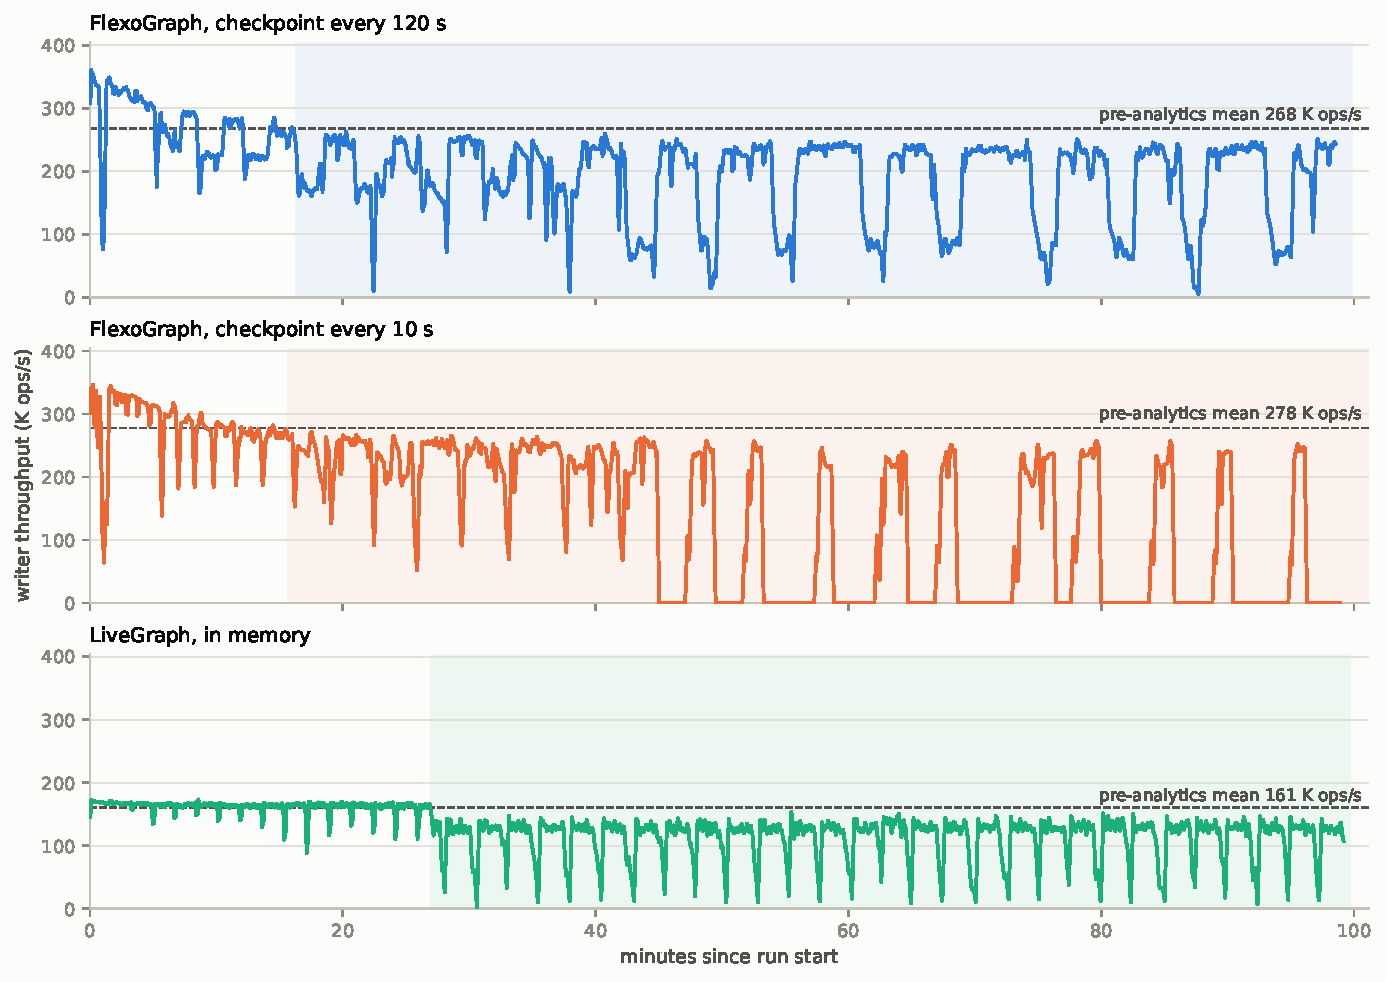
\includegraphics[width=\columnwidth]{fig/dynamic/concurrent_throughput_stacked.pdf}
  \caption{Writer throughput over time at $W=5$, one panel per run, drawn on shared axes.
  The tint marks each run's analytics window and the dashed line its own mean throughput before analytics began, so the gap between curve and line inside the tint is the loss that retention reports.
  \project{} at a $120$\,s checkpoint interval oscillates between peaks near its pre-analytics mean and deep troughs, and the pattern is the same at the end of the window as at the start.
  At the default $10$\,s checkpoint interval the same oscillation holds for the first half-hour of the analytics window, after which the troughs flatten at exactly zero and those flat stretches lengthen.
  LiveGraph oscillates in shallower, more frequent dips, steady throughout, at a lower absolute rate.}
  \label{fig:concurrent-throughput}
\end{figure}
%%%%%%%%%%%%%%%%%%%%%%%%%%%%%%%%%%%%%%%%%%%%%%%%%%%%%%%%%%%%%%%%%%%%%%%%%%%%%%%%

Two conclusions follow.
First, both systems retain close to $70\%$, and the $30\%$ they each lose measures the cost of running analytics alongside writers rather than the cost of checkpointing, because two designs with nothing in common land within a percentage point of each other.
Second, \project{} runs faster in absolute terms at this operating point, sustaining $267$\,K\,ops/s against LiveGraph's $161$ before analytics and $186$ against $113$ during it, while LiveGraph keeps nothing on disk.

Passes reuse checkpoints under this setting.
The $58$ passes read $14$ distinct checkpoints, about four passes to each, so a pass might read a graph that is a few minutes old.
Checkpoint duration also grew across the run, from $20$ seconds for the first to a plateau between $230$ and $342$ over the second half, and the peak update bytes closed to within $96\%$ of the conscription threshold.
We therefore claim this configuration holds for $100$ minutes, and we do not claim that it holds indefinitely.

\subsection{What each system writes to disk}
\label{sec:eval:dynamic:concurrent:io}

The comparison so far grants LiveGraph an advantage that is easy to overlook.
It holds the graph in anonymous memory, so nothing it does reaches a disk.
Its own persistence option is a file-backed block store, which it maps shared and leaves to the kernel to write back.
Running LiveGraph that way puts both systems on the same device, and sampling \texttt{/proc/diskstats} throughout each run measures what each one actually wrote (\autoref{tab:concurrent-io}).

%%%%%%%%%%%%%%%%%%%%%%%%%%%%%%%%%%%%%%%%%%%%%%%%%%%%%%%%%%%%%%%%%%%%%%%%%%%%%%%%
\begin{table}[t]
  \centering
  \setlength{\tabcolsep}{5pt}\renewcommand{\arraystretch}{1.05}
  \small
  \begin{tabular}{l r r r}
  \toprule
  Configuration & Retention & Written to device & Rate \\
  \midrule
  \project{}, checkpoint every $120$\,s & 69.0\,\% & 806\,GB & 168\,MB/s \\
  LiveGraph, file-backed block store    & 65.7\,\% & 1{,}049\,GB & 240\,MB/s \\
  LiveGraph, in memory                  & 70.3\,\% & none & none \\
  \bottomrule
  \end{tabular}
  \caption{Device-level write volume at $W=5$, taken from \texttt{/proc/diskstats} every $5$\,s.
  Both systems read almost nothing from the device, because neither runs under memory pressure.
  The in-memory configuration writes nothing by construction.}
  \label{tab:concurrent-io}
\end{table}
%%%%%%%%%%%%%%%%%%%%%%%%%%%%%%%%%%%%%%%%%%%%%%%%%%%%%%%%%%%%%%%%%%%%%%%%%%%%%%%%

LiveGraph writes more than \project{} does, not less.
The system with no checkpoints, no log, and no page reconciliation moved $1{,}049$\,GB to the device against \project{}'s $806$, and sustained $240$\,MB/s against $168$.
Write granularity explains the difference.
The kernel flushes every dirty mapped page once per expiry cycle, so a page that changes repeatedly gets written repeatedly, whereas a checkpoint reconciles each page once per interval however many times it changed.
LiveGraph's block file holds $155$\,GiB, so the run wrote roughly seven times the size of its own data.

Backing LiveGraph with a file also costs it throughput.
Its pre-analytics rate falls from $161$ to $146$\,K\,ops/s, its rate during analytics falls from $113$ to $96$, and its retention falls from $70.3$ to $65.7\%$.
The device is not the constraint, since $240$\,MB/s is about half what this SSD sustains.
The cost comes from the per-page work the kernel imposes: it write-protects each page after writing it back, so the next store to that page takes a fault, and it allocates file blocks on first touch.

Two qualifications belong with these numbers.
The two runs cover windows of $53.7$ and $40.3$ minutes, so their retention figures compare but their pass counts do not.
More importantly, a file-backed LiveGraph is storage-backed rather than recoverable: the kernel writes those pages in no particular order and flushes nothing until the mapping closes, so a crash leaves a torn file.
It buys a weaker guarantee than a checkpoint does, and it pays more I/O for it.

\subsection{Takeaway}
\label{sec:eval:dynamic:concurrent:takeaway}

Concurrent analytics over a checkpoint-based storage engine is checkpoint-bound.
The checkpoint that an analytics pass reads and the eviction that sustains the writers contend for the same B-tree, \wt{} resolves that contention in favour of the checkpoint, and the engine has one lever left: it stalls the writers, completely, for minutes at a time.

A schedule fixes this where a knob cannot.
Spacing checkpoints gives eviction time in which nothing bars it, and a low writer count keeps the dirty data small enough that eviction finishes within those gaps.
At that operating point \project{} sustains concurrent analytics at the same relative cost as an in-memory system, and it provides a consistent, crash-recoverable checkpoint that the in-memory system does not.

Two structural changes would attack the problem directly rather than scheduling around it: sharding the edge table so that the checkpoint bars eviction on one shard at a time, and a checkpointer that parallelises within a single tree.
Both remain future work.